% -----------------------------------------------------------------
% => BACKGROUND
% -----------------------------------------------------------------
\chapter{Conceitos e Definições}
\label{Chap:background}

Este capítulo faz uma contextualização teórica a partir de elementos utilizados na construção de ambientes de aprendizagem apoiados por tecnologia, tais elementos vão de novos paradigmas educacionais a áreas emergentes da Computação.

\section{Educação e práticas pedagógicas}\label{section:educacao_praticas}
Em nossa sociedade, a escola é a detentora oficial e formal dos mecanismos de validação do saber. Por isso, segundo ~\cite{Nogueira:2013}, em sua crítica à educação escolar, Bourdieu atenta para o problema de que a escola pode legitimar e reforçar as desigualdades sociais, caso não leve em consideração, em suas metodologias, a herança socialmente herdada pelos indivíduos que nela estudam. Desse modo, faz-se urgente e necessário buscar estratégias pedagógicas que diminuam o abismo entre o conhecimento oficialmente balizado e os capitais sociais e culturais dos estudantes economicamente menos favorecidos, para assim, colaborar mais eficazmente no seu êxito escolar.
 
\subsection{Educação, fracasso escolar e mudanças pedagógicas}\label{section:educacao_fracasso_mudancas}

Propor quaisquer modificações em metodologias pedagógicas ou processos educativos sem um questionamento prévio acerca do significado daquilo que está sendo feito, do contexto no qual se está inserido ou, ainda, sem considerar os diversos atores e elementos envolvidos nesses processos, pode contribuir ainda mais com o que se costuma chamar de ``fracasso escolar'' e que, para~\cite{Collares:1989}, tem fatores extra e intra escolares que precisam ser levados em consideração. Os fatores extra escolares são aqueles relacionados às condições de vida e subsistência, onde estudantes de classes mais pobres são prejudicados pelas péssimas condições econômicas, de saneamento básico, de moradia, alimentação e diversas outras privações.

Dentre os fatores intra escolares estão os programas de curso, os currículos, os trabalhos dos professores e os processos avaliativos. Para vários críticos da educação brasileira, dentre eles~\cite{Collares:1989} e~\cite{Perrenoud:2001}, o fracasso escolar depende mais dos fatores intra do que dos extra escolares. Todavia, para um melhor entendimento do problema, os fatores externos precisam estar articulados em relação aos internos, de modo que a caracterização do fracasso escolar deveria ser considerada menos como um problema de aprendizagem, isto é, vindo de deficiências do aluno, e mais como um problema de ``ensinagem'', vindo do sistema de ensino~\citep{Collares:1989}.

Pensar a melhoria e a eficiência da educação escolar a partir da necessidade de modificação dos processos educacionais, tem sido objeto de muitas análises ao longo dos anos, principalmente quando é feita uma crítica sociológica da educação, tal como pode ser constatado ao ler obras de pensadores como~\cite{charlot:2000}, \cite{Freire:1987} e Pierre Bourdieu~\citep{Nogueira:2013}. Destas leituras críticas, surgiram questionamentos e abordagens que levaram a novas concepções e tentativas de romper com um sistema concebido em uma época diferente da atual e que, por isso, já não consegue cumprir seu papel social. Assim, para uma educação de maior qualidade, é necessário reconhecer que o conhecimento é construído a partir da interação do indivíduo com o mundo ao seu redor e da significação que ele dá àquilo que o interpela, às atividades que executa e às interações sociais que estabelece com outros~\citep{charlot:2000}.

\subsection{Elementos do Processo de Ensino-Aprendizagem}

De acordo com~\cite{bassedas:1996}, o processo de aprendizagem, com interações complexas e variadas, possui pelo menos três elementos: (i) o estudante; (ii) os conteúdos de aprendizagem; e (iii) o professor. Sobre o estudante, pode-se retomar o pensamento de Pierre Bourdieu, onde cada indivíduo possui uma bagagem socialmente herdada, de modo que o sucesso escolar depende, em grande medida, de se levar em consideração os diversos tipos de capitais (econômico, social, cultural,...) que ele traz consigo para a escola~\citep{Nogueira:2013}. Em outras palavras, significa dizer que para um processo educativo ter êxito, é preciso que a escola adapte seus processos ao grupo ou ao indivíduo no contexto de aprendizagem. Além disso, tal adaptação precisa levar em consideração diversos elementos, dentre eles, o acesso aos conteúdos de aprendizagem.

\cite{Levy:2010}, ao discorrer sobre a Cibercultura, faz uma profunda discussão sobre a relação entre cultura, sociedade e técnica, apresentando a ideia de que esses três elementos são indissociáveis, mas, o fator humano é o mais preponderante, visto que, são as pessoas que produzem, utilizam e significam de diversos modos as diferentes técnicas.

Entretanto, \cite{Kenski:2007}, recorda que, por vivermos em um mundo imerso na tecnologia, estamos acostumados a certos confortos, como água encanada, luz elétrica, sapatos, Internet, e outros. Alguns desses elementos técnicos estão de tal maneira presentes na vida das pessoas que sua visão e significação do mundo passa necessariamente por essa base. Deste modo, um melhor proveito das novas tecnologias da informação no contexto educacional, exige que os conteúdos de aprendizagem não apenas estejam disponíveis nos dispositivos e canais de comunicação, mas, que usem linguagens e metodologias que verdadeiramente se comuniquem com os estudantes.

Seguindo o pensamento de~\cite{bassedas:1996}, não faz sentido pensar um processo de aprendizagem voltado para o êxito escolar do estudante sem tomar o professor como um elemento igualmente importante. De acordo com~\cite{Perrenoud:2001}, para que haja êxito escolar, o professor é o principal elemento a ser modificado. Por esse motivo, a inserção e a adaptação de recursos computacionais precisam levar em consideração a atuação e o papel do professor no contexto educacional, papel este que, gradativamente, migra de uma posição centralizadora, para uma postura de mediação.

O papel de mediador pressupõe o professor como um impulsionador da busca pelo conhecimento, que atue não como simples apresentador de conteúdo, mas, como agente de promoção de oportunidades que colaborem com o desenvolvimento do estudante, do seu pensamento crítico e da sua autonomia na busca pelo conhecimento~\citep{Chiovatto:2000}. Nesse sentido, a inserção de recursos computacionais no contexto de educação, implica em proporcionar ao docente um ambiente no qual ele se sinta seguro, livre e motivado a exercitar sua criatividade. Para que isso ocorra, é fundamental que as novas ferramentas e metodologias o façam sentir-se menos ameaçado com uma suposta perda de autoridade e centralidade, e mais empoderado com as oportunidades ação e intervenção~\citep{Perrenoud:2001}.

% %  O objetivo é trazer conceitos fundamenais relacionados a educação e à institucionalização da educação a partir da escola. Talvez, já entroduzir o conceito de Escola Tradicional que terá oposição na seção seguinte (onde serão abordados alguns elementos teóricos de Piaget, Paulo Freire, Bordieu e, talvez, Vygotsky).

\section{Teorias Sociopedagógicas}\label{section:sociopedagogicas}

Para realizar qualquer intervenção no processo de ensino-aprendizagem é preciso entender como ele acontece, por isso, é necessário adentrar na discussão sobre abordagens e concepções pedagógicas~\citep{bassedas:1996}.

\subsection{A Construção do Conhecimento a partir da Experiência}

De acordo com vários teóricos da educação, dentre eles, Seymour Papert, a inserção dos recursos computacionais no processo de ensino-aprendizagem pode colaborar com a urgente demanda de atualizar as metodologias educacionais~\citep{Almeida:2000}. Assim, nesta seção, serão apresentados alguns elementos das concepções e abordagens pedagógicas propostas por pensadores como Dewey, Paulo Freire, Piaget e Vygotsky que proverão fundamentos para a proposta apresentada neste trabalho.

\subsubsection{Método por Descoberta}

John Dewey propôs uma concepção de educação com base empírica a partir da aplicação do método científico, salientando a aquisição do conhecimento como um processo de reconstrução contínua a partir da reflexão sobre as experiências anteriores do indivíduo~\citep{Dewey:1971}.

Segundo~\cite{Almeida:2000}, o uso do método empírico envolve quatro etapas:
\begin{enumerate}
	\item \textbf{Ação:} experiência a partir de um objeto físico. 
	\item \textbf{Testagem:} reflexão para testar as hipóteses levantadas, o que permite encontrar outros objetos.
	\item \textbf{Depuração:} comparação entre os resultados obtidos e os esperados, a fim de corrigir os erros cometidos ou confirmar o que já se esperava.
	\item \textbf{Generalização:} transferência dos resultados a situações diferentes a partir da observação de novas experiências.
\end{enumerate}

Esta abordagem de Dewey leva em consideração que toda experiência humana decorre de interações e que é papel do professor compreender o processo de aprendizagem dos alunos, conhecendo seus interesses, necessidades, capacidades e experiências anteriores, para que possa propor ações que possibilitem novas interações e experiências significativas. Assim, tanto o professor, quanto o aluno precisam estar engajados como parceiros e assumindo uma postura de aprendizado~\citep{Almeida:2000}.

\subsubsection{Educação Emancipadora}

Paulo Freire critica a concepção dos processos de ensino-aprendizagem voltados a mera transmissão do conhecimento, considerando a acumulação deste por parte do aluno, como um `depósito' para uso futuro. Tal modelo é chamado por ele de educação bancária e é contraposto pela sua proposta pedagógica de caráter progressista e libertador~\citep{Freire:1987, Almeida:2000}.

A pedagogia proposta por Paulo Freire preocupa-se com que o aluno construa seu próprio conhecimento através da experiência direta, aprendendo a ler a palavra a partir do mundo~\citep{Almeida:2000}. Assim, para Freire, a escola precisa ser completamente modificada e atualizada, embora mantendo a sua condição de espaço-tempo que proporciona ``o conhecimento do conhecimento já existente'', a fim de se que possa produzir novos conhecimentos~\citep{Freire:1996}.

\subsubsection{Conhecimento como construção progressiva}\label{subsub:piaget}
De acordo com~\cite{Almeida:2000}, Piaget afirma que o conhecimento não é transmitido, mas, construído progressivamente a partir de interações entre o sujeito e seu meio. Assim, para Piaget, a inteligência é um recurso que possibilita a adaptação do sujeito ao meio, mas, que depende da combinação entre a assimilação e a acomodação.

Os processos de assimilação são caracterizados pela atuação do sujeito sobre um objeto, onde os elementos deste objeto são incorporados às estruturas existentes ou em formação no sujeito. Já os processos de acomodação estão relacionados a atuação do sujeito sobre si próprio, a partir da transformação que os elementos assimilados provocam no próprio sujeito. Assim, o conhecimento é construído no processo de adaptação do sujeito que acontece no equilíbrio entre a assimilação e a acomodação, a partir da interação com um objeto~\citep{Almeida:2000}.

Tendo isso como pressuposto, seria função dos processos pedagógicos promover interações (experimentações) entre o sujeito e os objetos que favorecessem a construção progressiva das estruturas de inteligência a partir da reflexão e da descoberta. No contexto desta tese, será proposto um ambiente e um modelo para integração de manipulativos tangíveis de aprendizagem que possibilitem experiências que promovam a construção do conhecimento por parte dos estudantes.

\subsubsection{Zona de Desenvolvimento Proximal}
Vygotsky propôs a teoria histórico-social onde afirma que o conhecimento é edificado e construído a partir dos contextos sociais da aprendizagem~\citep{Vygotsky:1998}. Assim, fica evidenciada a importância da cultura na aprendizagem, pois, é a cultura que determina quais habilidades e saberes são necessárias para estar socialmente presente na e com a sociedade.

\cite{Rego:2013} afirma que para que a aprendizagem aconteça é fundamental que se tenha: (a) mediação, (b) linguagem, (c) processo de internalização e (d) níveis de desenvolvimento. Destes quatro elementos, destacamos a mediação e os níveis de desenvolvimento, onde, no primeiro momento, a relação do ser humano com o mundo, e consequentemente sua aprendizagem, é entendida como uma relação mediada por objetos, símbolos, outro ser humano ou elementos. Nessa perspectiva, o papel social do professor e da tecnologia é o de mediar o processo de aprendizagem.

Além disso, é preciso considerar que, pela teoria histórico-social, o ser humano possui um nível de desenvolvimento atual e um nível potencial. O atual tem relação com aquilo que o estudante já conhece e, portanto, sabe fazer por conta própria, isto é, o conhecimento já construído, enquanto o potencial diz respeito às possibilidades de conhecimento a ser construído. Assim,~\cite{Vygotsky:1998} infere a existência de uma distância entre os níveis de desenvolvimento atual e potencial, a qual chama de Zona de Desenvolvimento Proximal (ZDP). %e que ``define aquelas funções que ainda não amadureceram, mas que estão em processo de maturação, funções que amadurecerão, mas que estão, presentemente, em estado embrionário"~\cite{Vygotsky:1998}.

Desse modo, o professor deve conhecer o que cada aluno já traz consigo e o que poderá construir para, assim, identificar a ZDP de cada um e atuar adequadamente no processo de aprendizagem, ajudando no estabelecimento de novas as estruturas e conhecimentos~\cite{Almeida:2000}. Assim, é importante salientar que a inserção das novas tecnologia nos processos educacionais pode auxiliar o professor tanto na identificação quanto na criação da ZDP, além de permitir um nível de autonomia do estudante no processo de busca e construção do conhecimento.

No contexto desta tese, além dos objetos de aprendizagem tradicionais e dos manipulativos tangíveis, serão apresentadas métricas que possibilitem a avaliação e o acompanhamento da aprendizagem dos estudantes, de modo a fornecer aos entes envolvidos no processo de ensino-aprendizagem mais elementos que auxiliem na percepção do que precisa ser apreendido pelos estudantes.

%AVISO
%------ TERMINAR DE ESCREVER ----%

%A ideia é embasar a adaptação da escola aos tempos atuais a partir da crítica de alguns teóricos da educação como Piaget, Paulo Freire, Bordieu e, talvez, Vygotsky


%----------------------------------


%\section{Informática na Educação}
%      Por que usar computadores na educação? 
%      Breve introdução ao tema da inserção de computadores no processo de ensino. 
%      Reforço da distinção entre uma disciplina sobre como usar o computador e o computador como instrumento de fato. 

%\subsection{Aprendizado apoiado por Tecnologia}
%   Sociedade digital. Cibercultura, ciberespaço, possibilidades de interação com o mundo virtual para construção ou aquisição de conhecimento, algo sobre interação físico-virtual?
%   Dispositivos Móveis, Android, Tecnologia Web.

\section{Computação Aplicada à Educação}\label{section:computacao_educacao}

A Educação 4.0, pressupõe que a computação facilite e aprimore os processos educacionais, alterando drasticamente os diversos elementos pedagógicos, seja o ambiente de sala de aula, seja as atividades de aprendizagem ou seja os mecanismos de avaliação e acompanhamento. Desse modo, o principal objetivo de aliar o uso de dispositivos móveis, sensores, Internet das Coisas e sistemas ciber-físicos aos processos educacionais é colaborar com que as diversas situações de  ensino-aprendizagem sejam mais interessantes e eficientes.

Nesta Tese, a essa integração entre sala de aula e tecnologia denominamos Educação Digital e alguns conceitos relacionados são apresentados a seguir.

\subsection{Objetos de Aprendizagem}
Seja em processos educativos mais tradicionais, seja onde há primazia da autonomia do estudante na construção do conhecimento, a inserção das novas tecnologias na educação tem demandado a geração de diversos materiais educacionais~\citep{Tarouco:2004}.

Esses materiais são o que chamamos de ``Objetos de Aprendizagem'' (OA) e podem ser categorizados, armazenados, distribuídos ou reusados e sempre estão atrelados a educação apoiada por tecnologia. Sendo assim, são considerados objetos de aprendizagem: imagens, gráficos, vídeos, áudios, \textit{slides} ou qualquer outra ferramenta ou recurso digital com finalidade educacional que contenha informações sobre o contexto de utilização~\citep{Tarouco:2004}.

Além da \textbf{reusabilidade}, OAs possuem ainda as seguintes características: \textbf{(i) acessibilidade:} possível de ser usado remotamente e simultaneamente em diversos lugares; \textbf{(ii) portabilidade:} um recurso produzido em um local e com uma ferramenta pode ser usado em outro local com outra ferramenta; \textbf{(iii) modularidade:} um objeto pode estar contido em outro, podendo ser combinados; \textbf{(iv) autossuficiência:} um objeto não depende de outros para fazer sentido; \textbf{(v) metadados:} são descritos por metadados como nome do autor, data, idioma, objetivos educacionais~\citep{Tarouco:2004,Sabbatini:2013}.

Considerando que um objeto de aprendizagem é um recurso didático (vídeo, slide, áudio, imagem, etc) a ser inserido no processo educativo, a composição e a efetiva utilização destes objetos em um sistema ou ambiente de ensino-aprendizagem faz parte do que chamamos de aula. No contexto desta proposta, esses objetos seriam acionados e utilizados de acordo com a necessidade e visando a interação do estudante com o sistema. Assim, %expandindo o exemplo da Seção~\ref{sub:contextawareness} sobre Ciência de Contexto, diferentes objetos poderiam ser acionados 
de acordo com os objetivos de aprendizagem, um estudante pode interagir com diferentes objetos de aprendizagem que o ajudem a construir conhecimentos e a desenvolver competências e habilidades específicas.

Nesse contexto, o estudo de~\cite{Salehi:2014} indica que o uso de manipulativos físicos pode aumentar significativamente os ganhos de aprendizagem quando comparados a simulações em ambientes virtuais. Assim, o uso de objetos de aprendizagem que sejam, ao mesmo tempo, físicos e digitais deve não somente expandir as possibilidades de construção do conhecimento, mas, também aumentar o engajamento dos estudantes. Nas seções~\ref{section:iot}, \ref{section:ciberfisico} e \ref{section:TUI}, são apresentados elementos que agregam mais informação ao tipo específico de objeto de aprendizagem que dá o enfoque deste trabalho.

\textbf{Padrões de Metadados de OAs}

Para tornar a criação e o uso dos diversos Objetos de Aprendizagem mais fácil, muitos grupos de pesquisa e entidades tem proposto padronizações dos metadados~\citep{vicari:2009}. Esta busca por padronização tem como principal objetivo facilitar a pesquisa, avaliação, aquisição e o uso de tais objetos por parte dos estudantes, professores e softwares automatizados, bem como permitir o desenvolvimento de repositórios de objetos que levem em consideração os diversos contextos culturais nos quais os objetos podem ser reutilizados~\citep{learning2002ieee}.

De acordo com~\cite{mcclelland:2003}, os dois padrões mais populares são \textit{Dublin Core Metadata Element Set} e \textit{IEEE Learning Object Metadata}. Assim, neste trabalho, focaremos no IEEE-LOM (\textit{Learning Object Metadata}) por ser um padrão aberto e internacionalmente reconhecido, que segue a norma IEEE Std 1484.12.1 - 2020, sendo normalmente codificado em XML. Além disso, existe uma extensão brasileira para o padrão IEEE-LOM, disponibilizada por~\cite{vicari:2009}, cujo  objetivo é apresentar um padrão para objetos de aprendizagem que seja multiplataforma (em especial, \textit{Web}, TV Digital e dispositivos móveis), que suporte requisitos de acessibilidade e que disponibilize informações educacionais específicas do contexto brasileiro. Tal extensão é chamada de OBAA (Objetos de Aprendizagem Baseados em Agentes) e também possui um modelo básico para sintaxe e semântica dos metadados, através da especificação de uma ontologia OWL para os mesmos~\citep{vicari:2009}.

Desse modo, após um estudo dos padrões OBAA e IEEE-LOM, selecionamos um perfil de metadados que seja razoavelmente compatível com a proposta desta tese (disponível no Apêndice~\ref{Chap:AppendixA}).
%, mas que ainda assim precisará ser estendido para abarcar os objetos físico-virtuais de aprendizagem.

%\subsection{Aprendizagem Ubíqua}
%
%O desenvolvimento de ambientes de aprendizagem ubíqua se baseia no conceito de computação ubíqua (ou pervasiva) que é o uso de dispositivos embarcados, computadores vestíveis (sapatos, roupas, relógios, etc) e dispositivos móveis conectados por rede de comunicação sem fio~\citep{Yau:2003}.
%
%O termo "computação ubíqua"~significa que a computação existe "em torno de nós", "em todos os lugares", assim, quando aplicado à aprendizagem, quer dizer que o espaço de informação e o espaço físico são convergentes. Sendo assim, as demandas e os recursos de aprendizagem estão por toda parte e os estudos, a vida e o trabalho estão interligados \citep{Oluwagbemi:2014,Xue:2011}.
%
%De acordo com~\cite{Ogata:2005}, as principais características de ambientes de aprendizagem ubíqua são:
%\begin{itemize}
%	\item \textbf{Permanência:} os estudantes nunca perdem seus trabalhos, a não ser que sejam propositalmente apagados e, todo o processo de aprendizagem é gravado.
%	\item \textbf{Acessibilidade:} os estudantes tem acesso aos seus documentos, dados ou vídeos em qualquer lugar. A informação provida é baseada nas requisições feitas por ele, isso faz com que o aprendizado seja auto direcionado.
%	\item \textbf{Imediatismo:} onde o estudante estiver pode obter quaisquer informações imediatamente. Assim, podem resolver problemas rapidamente.
%	\item \textbf{Interatividade:} os estudantes podem interagir com especialistas, professores ou colegas síncrona ou assicronicamente.
%	\item \textbf{Situação de atividades de instrução:} o aprendizado pode ser embutido na própria vida do estudante. Tanto os problemas encontrados, quanto o conhecimento necessário pra resolvê-los, são apresentados de maneira natural e autêntica.
%\end{itemize}
%
%\subsection{Inteligência de Ambientes (AmI)}
%
%De acordo com~\cite{Margetis:2011}, a maior parte das pesquisas envolvendo ambientes inteligentes é relacionada ao desenvolvimento de casas inteligentes ou ambientes de escritório colaborativos. Entretanto, quase não se tem usado essa abordagem na criação de salas de aula inteligentes.
%
%Tal como a computação ubíqua ou pervasiva, AmI parte do pressuposto da integração em rede entre os dispositivos embarcados para criar um cenário em que os processos computacionais não sejam claramente percebidos pelas pessoas. Adicionalmente, a interação com a tecnologia deve ser tão amigável que o usuário se perceba naturalmente capacitado para seu uso, além de um serviço de suporte mais efetivo~\citep{Li:2009}.
%
%Segundo~\cite{Li:2009}, um AmI é constituído de quatro características:
%\begin{itemize}
%	\item \textbf{Embarcação:} capacidade computacional embutida em todos os dispositivos que devem se comunicar em rede;
%	\item \textbf{Personalização:} dispositivos e dados nos dispositivos são direcionados ao uso pessoal;
%	\item \textbf{Adaptação:} os dispositivos devem se adaptar a pessoa que o está utilizando ou ao contexto em que está sendo usado;
%	\item \textbf{Antecipação:} os dispositivos devem antecipar o comportamento preferido e começar a se comportar de acordo com ele sem a necessidade de se dizer explicitamente para fazer isso.
%\end{itemize}
%
%
%\subsection{Ciência de Contexto}\label{sub:contextawareness}
%
%Para ser minimamente intrusivo, um sistema de computação pervasiva precisa ter ``ciência de contexto'', isto é, ele precisa: (i) reconhecer o estado atual do usuário; (ii) modificar seu comportamento a partir do conhecimento desse estado. O estado (ou contexto) de um usuário pode ter diversas características, tais como localização geográfica, orientação geoespacial, estado fisiológico, emocional ou histórico de comportamento ou preferências, entre outros. Diante do conhecimento do estado atual, o sistema pode se antecipar e tomar decisões em prol de auxiliar o usuário, com um tipo de assistente pessoal~\citep{Satyanarayanan:2001}.
%
%Um exemplo de ciência de contexto é um aplicativo que, tendo informação do componente curricular que está sendo abordado na escola, ofereça sugestões de eventos culturais relacionados. Assim, um aluno que está estudando sobre Ciclo da Borracha e, nesse período, passa próximo a um teatro em que está em cartaz um musical sobre esse tema, pode ser automaticamente notificado e receber informações sobre horários e valores de ingressos. Caso ele compre o ingresso para um sessão em um horário diferente do atual e receba essa informação por email, o sistema pode salvar o compromisso na agenda e, quando chegar o momento, traçar a melhor rota para o teatro supondo o meio de transporte mais usado por ele.
%
%Assim, para melhor apoiar o aprendizado do estudante, é necessário que o ambiente de aprendizagem se adapte a ele. Por esse motivo, o sistema precisa reunir e analisar informações relacionadas ao estudante e ao ambiente físico no qual ele está atualmente inserido. A partir dessa percepção, o sistema pode fazer recomendações mais adequadas e que auxiliem positivamente no processo de aprendizagem~\citep{Li:2009,Crompton:2015}
%
\subsection{Internet das Coisas (IoT)}\label{section:iot}

Para~\cite{Vermesan:2013}, a Internet das Coisas é um conceito e um paradigma que considera uma variedade de coisas e objetos presentes em um ambiente geral, ligadas por meio de fios ou recursos sem fios e são capazes de interagir uns com os outros e cooperar com outras coisas e objetos com o objetivo de criar novas aplicações e/ou serviços e alcançar objetivos comuns.

De acordo com~\cite{Chang:2014}, do ponto de vista da estrutura, cenários baseados em IoT podem ser divididos em quatro camadas:

\begin{itemize}
	\item \textbf{Camada de Percepção:} composta por sensores (i.e.: acelerômetro, giroscópio,...), aparelhos inteligentes (i.e.: smartphones) e etiquetas (i.e.: RFID (\textit{Radio-Frequency IDentification}), Códigos de Barra, \textit{QR Code}), ou seja, tecnologias que permitam coleta de dados ou identificação.
	\item \textbf{Camada de Rede:} camada de conexão e transferência de dados. Ela é composta por tecnologias de comunicação em rede (ie: 3G, 4G, WiFi, \textit{Bluetooth}, \textit{ZigBee}, Infravermelho);
	\item \textbf{Camada de Processamento:} tem a função de coletar, tratar e analisar os dados adquiridos pelos sensores (ie: Compressão de Dados, Cache de Dados, Computação);
	\item \textbf{Camada de Aplicação:} camada de interface com o usuário responsável por armazenar ou minerar dados, recursos de conteúdos, aplicações de ensino, entre outros.
\end{itemize}

Além disso,~\cite{serbanati:2011} definem o paradigma da Internet das Coisas de modo mais amplo ao afirmar que é uma visão da conexão entre o digital e o físico em um mundo ``aumentado'' no qual usuários (humanos ou não) cooperam para atingir seus objetivos. Assim, para concretizar este paradigma, as seguintes características deveriam estar progressivamente presentes nas infraestruturas de rede de modo a proporcionar a integração entre os mundos físico e digital: (i) identificação de objetos e detecção de presença; (ii) captura autônoma de dados; (iii) associação de identificação(ID) automática para recursos; (iv) interoperabilidade entre diferentes tecnologias de comunicação; (v) transferência de evento; (vi) interação baseada em serviço entre objetos; (vii) comunicação baseada em semântica entre objetos; (viii) cooperação entre objetos autônomos.

\begin{figure}[htb]
	\centering
	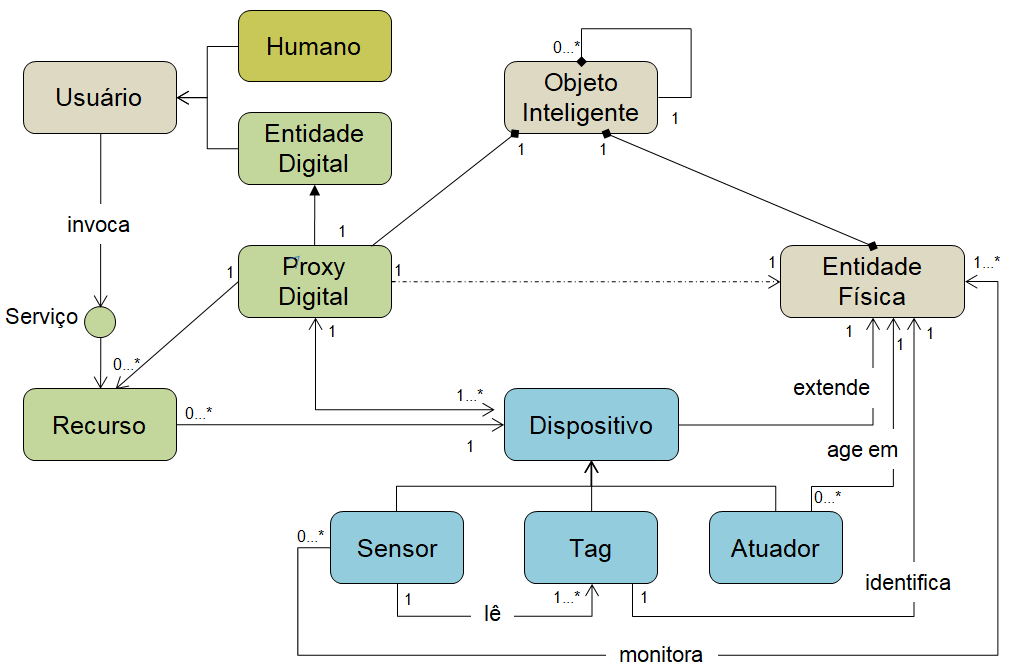
\includegraphics[width=0.9\linewidth]{chapters/background/arquitetura_IoT.png}
	\caption{Modelo de Referência para IoT. Fonte:~\cite{serbanati:2011}}
	\label{fig:modeloiot}
\end{figure}

Assim,~\cite{serbanati:2011} apresentam um modelo de referência para IoT (Figura~\ref{fig:modeloiot}) que define ``Entidades Físicas'' e ``Entidades Digitais'', onde as entidades físicas podem ser quaisquer objetos ou ambientes (de humanos a dispositivos eletrônicos ou ambientes fechados/abertos) discretos e identificáveis que sejam de interesse do usuário e o ajudem a alcançar a sua própria meta, e as digitais são ``entidades de \textit{software} que podem ser agentes com objetivos autônomos, serviços ou entradas de dados coerentes''. Além disso, as entidades digitais podem interagir tanto entre si quanto com os usuários e, no mundo digital, podem representar entidades físicas, nesse caso, como um ``\textit{Proxy} Digital''.

\cite{serbanati:2011} esclarecem que as representações digitais de Entidades Físicas podem ser de diversos tipos, dentre eles: modelos 3D, avatares, objetos (ou instâncias de uma classe em uma linguagem de programação orientada a objetos) e, até mesmo uma conta de rede social pode ser vista como tal. Entretanto, no contexto da IoT, de acordo com~\cite{serbanati:2011}, Proxies Digitais tem duas propriedades fundamentais:

\begin{itemize}
	\item Cada \textit{Proxy Digital} \textbf{representa biunivocamente uma única Entidade Física} e, por isso, contém apenas um ID para identificar o objeto representado. Além disso, a associação entre o Proxy Digital e a Entidade Física representada deve ser estabelecida automaticamente;
	\item Um \textit{Proxy Digital} é uma \textbf{representação sincronizada de um conjunto de propriedades da Entidade Física}. Assim, os parâmetros digitais relevantes que representam as características da Entidade Física podem ser atualizados de acordo com qualquer mudança observada no estado da entidade física (i.e.: através de sensores). De modo análogo, as alterações que afetam o Proxy Digital podem se manifestar na Entidade Física (i.e.: através de atuadores).
\end{itemize}

A extensão de uma Entidade Física e do \textit{Proxy} Digital associado a ela é definida por~\cite{serbanati:2011} como ``\textit{Objeto Inteligente}'', sendo necessário que \textit{Dispositivos} façam essa integração de modo que ``quaisquer mudanças nas propriedades de um objeto inteligente devem ser representadas tanto no mundo físico quanto no digital''.

Assim, do ponto de vista funcional, tais Dispositivos podem ser de três tipos: (i) \textbf{Sensores}, que proveem informações sobre a Entidade Física que eles monitoram; (ii) \textbf{Tags} (código de barra, QRCode, RFID,...), que podem dar suporte ao processo de identificação; e, (iii) \textbf{Atuadores}, que podem modificar o estado físico da Entidade Física. 

Além dos componentes mencionados anteriormente, no Modelo de Referência para IoT apresentado na Figura~\ref{fig:modeloiot}, podem ser observados outros dois elementos: (a) ``Recurso'' e (b) ``Serviço''. Onde, Recursos são componentes digitais que podem prover cinco capacidades diferentes: (1) recuperação ou modificação das propriedades físicas de uma Entidade Física associada, por meio de sensores ou atuadores; (2) modificação ou recuperação de propriedades digitais de um Proxy Digital associado; e (3) uso de serviços de hardware complexo ou de software através do objeto inteligente associado. E, por fim, Serviço é o meio pelo qual os recursos são efetivamente acessados para minimizar a dependência que as implementações tem em relação ao  \textit{hardware}.

É importante salientar que, no contexto deste trabalho, o uso de elementos de IoT diz respeito às relações e às interações que os componentes físicos e digitais precisam estabelecer e que são expressas através de modelos computacionais já estabelecidos como os apresentados nos trabalhos de~\cite{Chang:2014} e~\cite{serbanati:2011}.

% \subsection{Sistemas multiagente}
% Segundo~\cite{bez:2012}, sistemas multiagente são sistemas com múltiplos agentes com (i) comportamento autônomo e que (ii) interagem uns com os outros, sendo essas, suas duas características básicas. Além disso, cada agente é um elemento autônomo que trabalha independentemente dos outros agentes, assim, um sistema multiagente é um sistema computacional que coordena as habilidades dos diversos agentes individuais para resolver problemas ou satisfazer um conjunto de tarefas ou objetivos~\citep{bez:2012}.

% No que diz respeito à categorização, existem dois tipos de sistemas multiagente: reativo e cognitivo. Os sistemas do tipo reativo apenas respondem a estímulos ambientais, sem qualquer tipo de modelo do ambiente ou memória das ações e possuem grande número de agentes. O sistemas cognitivos tem poucos agentes, pois, cada agente é um sistema complexo e computacionalmente caro. Nesses sistemas, os agentes raciocinam e deliberam em conjunto quais ações ou planos devem ser executados e quais objetivos serão alcançados, além de manter históricos das interações passadas~\citep{giuffra:2012,ferber:1991}. 

% Em um ambiente de aprendizagem que também tenha, por exemplo, ciência de contexto, um sistema multiagente será o responsável pela percepção das sensações ambientais, reconhecimento de determinado estado do usuário e deliberação das recomendações ou ações que gerem adaptações que permitam personalização da experiência de ensino-aprendizagem. Os trabalhos inicialmente encontrados nessa área e aplicados à educação digital não utilizavam sistemas multiagente em sistemas ciber-físicos para intervenção e adaptação de conteúdo no decorrer do processo educacional.

\subsection{Sistemas Ciberfísicos}\label{section:ciberfisico}
O termo ``sistemas ciberfísicos'' foi proposto por Helen Gills para definir sistemas físicos, biológicos e de engenharia, cujas operações são integradas, monitoradas e/ou controladas por um núcleo computacional e os seus componentes estão conectados~\citep{wade:2015}. Esse termo está substituindo o famoso ``Sistemas Embarcados'', pois, enfatiza de modo mais evidente sua interação com o mundo físico~\citep{helps:2013}.

Segundo~\cite{chase:2011}, por estarem diretamente conectados ao ambiente físico, sistemas ciberfísicos tem como principais características: (i) confiáveis: não podem falhar; (ii) seguros: não pode causar dano ao ambiente e à vida que nele habita (iii) restrição de tempo: processamento de dados dentro de um pequeno limite temporal, pois, as notificações e tomadas de decisões, em determinadas circunstâncias, precisam ser imediatas.

Diversos trabalhos usando sistemas ciberfísicos tem surgido a partir das necessidades de melhoria nos processos de ensino-aprendizagem, ora focando no ensino de Engenharia, ora focando em aprendizagem colaborativa e ambientes adaptativos ou ainda na criação de extensões de ambientes virtuais~\citep{Santos:2014,lei:2013,wade:2015,noor:2011,pester:2015,peter:2015}.

Assim, tendo enfoque na construção de um ambiente ciberfísico de aprendizagem, \cite{santos:2014ambientes} propõe oito requisitos para a construção desses ambientes: (i) prover \textbf{comunicação e interação} entre estudantes e professores com vistas a possibilitar a aprendizagem colaborativa; (ii) possuir \textbf{ferramentas administrativas} para gerência educacional; (iii) possuir \textbf{ferramentas de avaliação} da aprendizagem; (iv) possibilitar diferentes \textbf{abordagens pedagógicas}; (v) possuir \textbf{ferramentas de autoria} que possibilitem a criação ou edição de conteúdos educacionais; (vi) possuir algum nível de \textbf{inteligência} para o auxílio da aprendizagem; (vii) proporcionar maior \textbf{engajamento} através de experiências participativas; (viii) deve ter uma \textbf{abordagem multissensorial} que integre informações dos ambientes, tais como sons, vídeos, textos e animações 3D, entre outras.

No contexto desta teste, um sistema ciberfísico implica na inserção e utilização de objetos de aprendizagem que sejam simultaneamente físicos e digitais em um ambiente de aprendizagem tal como outros objetos tradicionais, i.e. slides, vídeos, imagens, simulações, entre outros, o que implica na necessidade de mecanismos de controle (atuadores) e de percepção (sensores). Além disso, o ambiente de aprendizagem deve possibilitar coleta de dados de interação dos alunos durante a utilização desses objetos tangíveis e deve fornecer instrumentos para posterior análise dos dados, avaliação/acompanhamento da aprendizagem e propostas de intervenção pedagógica nos processos de ensino-aprendizagem dos estudantes.


% No contexto desta proposta, após a aula, um sistema ciber-físico pode recomendar atividades pedagógicas com objetos de aprendizagem físico-virtuais levando em consideração as dificuldades específicas de um aluno, percebidas pelo sistema, com relação a algum aspecto do conteúdo didático. Nenhum dos trabalhos encontrados que utilizam sistemas ciber-físicos em contextos educacionais utilizavam uma abordagem muiltiagente aliada a análise de dados educacionais dos alunos para tomada de decisões no sentido de adaptar conteúdo educacional ao estilo de aprendizagem ou à necessidade de reforço didático do estudante.
	
	
% \subsection{Ambientes de Sala de aula inteligente}

% Enquanto ~\cite{Gligoric:2012} considera que uma sala de aula inteligente é uma sala de aula que provê, em tempo real, \textit{feedback} automático, por exemplo, sobre a qualidade da aula, podendo também ser um ambiente inteligente equipado com diferentes tipos de \textit{hardware} e \textit{software}, para~\cite{Bargaoui:2014}, o que caracteriza esses ambientes é o fato de eles serem projetados de modo a permitir o controle dos equipamentos audiovisuais, computadores, projetores, lousas interativas com o objetivo de facilitar a interação entre professores e alunos.

% Assim, a leitura de diversos trabalhos relacionados, aponta para a percepção de que uma sala de aula inteligente é caracterizada pela inserção de dispositivos computacionais como \textit{tablets}, lousas inteligentes ou sensores diversos que possibilitem maior interatividade e algum nível de inferência para recomendações ou notificações ao professor ou ao aluno, utilizando elementos de computação pervasiva ou Internet das Coisas~\citep{Margetis:2011,Santana:2013,Dekdouk:2012}.

% Outra interpretação de sala de aula inteligente pode ser feita a luz de trabalhos focados na construção de Ambientes Virtuais de Aprendizagem (AVA). Assim, alguns dos trabalhos relacionados a AVA apresentam arquiteturas e implementações, baseadas em tecnologia Web ou de dispositivos móveis, para proporcionar interação virtual entre os alunos~\citep{Monteiro:2015} ou ambientes de aprendizagem colaborativa~\citep{Brito:2002,Netto:2003}.

% %Se a inserção de recursos computacionais tem como objetivo principal apoiar e facilitar os processos de ensino-aprendizagem e, assim, garantir uma maior qualidade na educação, então, uma sala de aula inteligente não pode ser esquivar de levar em consideração o modo retemos conhecimento.

% %\begin{figure}[h]
% %	\centering
% %	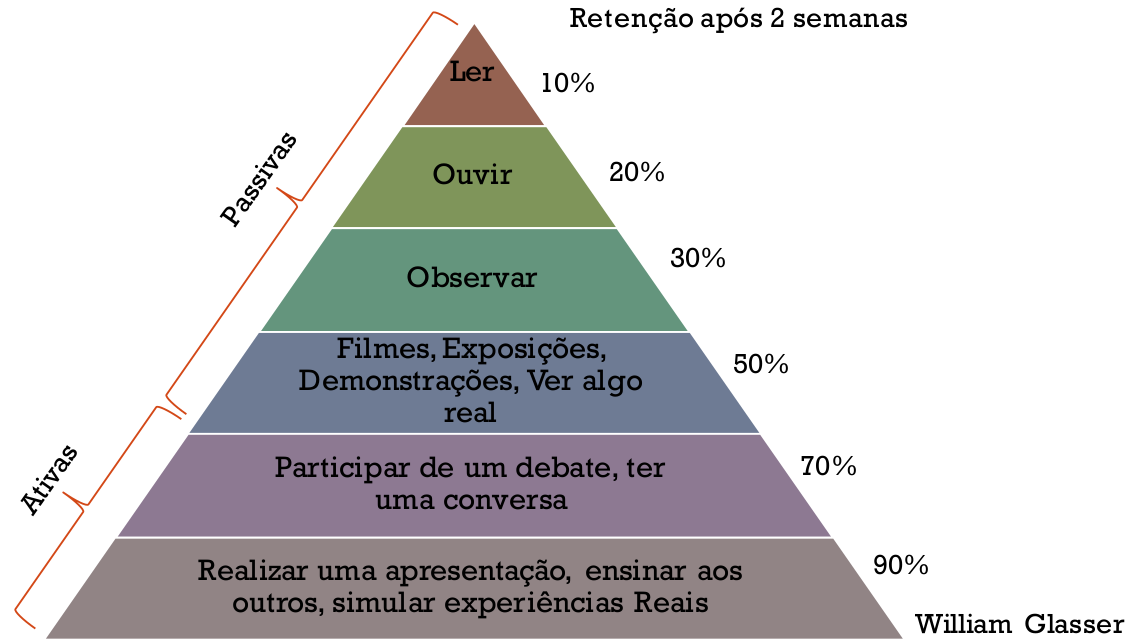
\includegraphics[width=0.7\linewidth]{imgs/piramide_glasser}
% %	\caption{Como aprendemos - Pirâmide de Glasser}
% %	\label{fig:piramide_glasser}
% %\end{figure}

% %  Conceito de sala de aula inteligente, possibilidades de aquisição de dados de sensores, dados de interação com o conteúdo educacional, possibilidades de inferências, recomendações ou notificações com relação às dificuldades ou potencialidades da turma ou de um aluno específico.
% %
% %Apresentar elementos sobre retenção de conhecimento a partir da pirâmide de William Glasser (apresentação do Tiago Primo) e como a educação apoiada por tecnologia pode ajudar nisso(quanto mais ativa aprendizagem, mais conhecimento é retido). Apresentar o conceito de sala de aula inteligente como um caminho para maior engajamento do estudante e retenção quando unido com atividades de aprendizagem ativa.



\subsection{Interfaces Tangíveis de Usuário}\label{section:TUI}

\cite{ishii:1997} introduziram o conceito de ``Interfaces Tangíveis de Usuário'' (do inglês, \textit{Tangible User Interfaces} - TUIs) como um novo tipo de Interface Humano-Computador (IHC) que permite ao usuário interagir com um sistema computacional através de objetos e ambientes físicos do dia-a-dia, ao invés de utilizar periféricos tradicionais como mouse, teclado e monitor em conjunto com uma Interface Gráfica de Usuário - GUI (Figura~\ref{fig:guiandtui}).

\begin{figure}[htb]
	\centering
	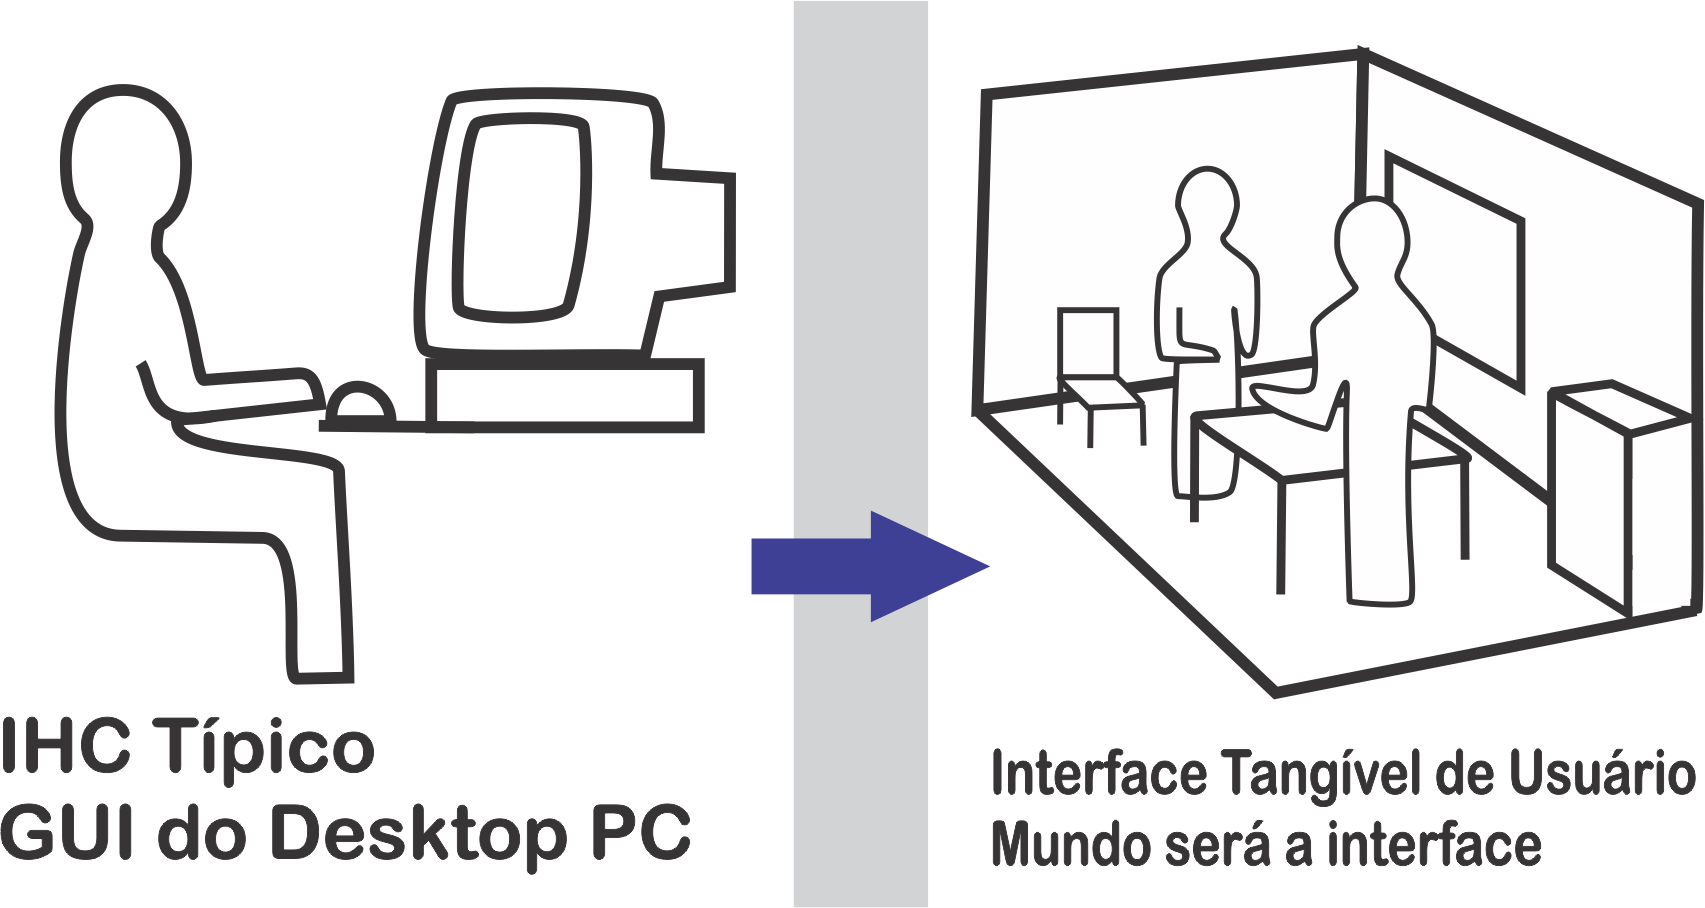
\includegraphics[width=0.7\linewidth]{chapters/background/GUIandTUI_redesenhado.png}
	\caption{GUI e TUIs. Fonte:~\cite{ishii:1997}}
	\label{fig:guiandtui}
\end{figure}

Segundo \cite{ullmer:2000}, interfaces tangíveis de usuário dão forma física à informação digital de modo que os objetos físicos servem como representações ou controles físicos para a mídia computacional. Assim, essas representações físicas (tangíveis) são combinadas com representações digitais (intangíveis e transitórias) resultando em sistemas fisicamente interativos, mas, mediados computacionalmente. Para um melhor entendimento, \cite{ullmer:2000} fornecem a seguinte heurística: quando a força/energia de uma interface tangível é desligada, as representações digitais desaparecem e as representações físicas persistem, de modo que ``as interfaces tangíveis são produtos de um cuidadoso equilíbrio entre essas duas formas de representação''.

\begin{figure}[htb]
	\centering
	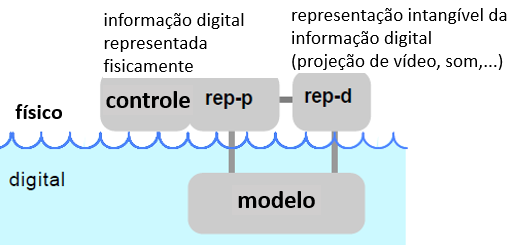
\includegraphics[width=0.6\linewidth]{chapters/background/MCRpd_2.png}
	\caption{Modelo de interação de TUI - MCRpd. Fonte:~\cite{ullmer:2000}}
	\label{fig:MCRpd}
\end{figure}

Assim, baseando-se no padrão que serviu de modelo tradicional para construção de interfaces gráficas de usuário (\textit{model-view-controller}), onde a interação humana acontece basicamente através de `entrada' (por meio de periféricos como mouse e teclado) e `saída' (representações digitais como gráficos e texto baseados em tela), \cite{ullmer:2000} apresentam um modelo de interação para interfaces tangíveis que denominam de \textit{model-control-representation (physical and digital)} (MCRpd), onde os elementos ``modelo'' e ``controle'' são mantidos e o elemento \textit{view} foi dividido em dois subcomponentes: representações físicas (``rep-p'') e representações digitais (``rep-d''), conforme a Figura~\ref{fig:MCRpd}.

Segundo~\cite{ullmer:2000} e~\cite{zhou:2015}, o modelo de interação intangível destaca quatro características chave das interfaces tangíveis: 
\begin{enumerate}
	\item As representações físicas (`rep-p') são acopladas computacionalmente aos dados digitais subjacentes (`modelo')
	\item As representações físicas incorporam mecanismos de controle físicos interativos (`controle'), permitindo ao usuário a manipulação de objetos.
	\item As representações físicas são acopladas perceptivamente às representações digitais (`rep-d').
	\item O estado físico dos objetos tangíveis incorpora parcialmente o estado digital do sistema, de modo que, o sistema é, pelo menos, parcialmente legível se a energia for cortada.
\end{enumerate}

%Objetos tangíveis são acoplados a dados digitais por meio de funcionalidade computadorizada.
%Interação manual com objetos tangíveis: os objetos tangíveis incorporam os meios de controle interativo, permitindo ao usuário manipular objetos.
%Os objetos tangíveis são acoplados perceptivamente com a representação produzida digitalmente.
%O estado dos objetos tangíveis incorpora aspectos centrais do estado de todo o sistema (significado representacional), e o sistema é, portanto, pelo menos parcialmente legível se a energia for cortada.

\textbf{Interfaces Tangíveis na Educação}

No últimos anos, diversos trabalhos tem apresentado interfaces tangíveis aplicadas ao ensino-aprendizagem, assim foram propostos principalmente trabalhos envolvendo mesas tangíveis \citep{mendoza:2019, ishii:1997}, blocos para programação tangível \citep{panaggio:2019, carbajal:2018, leite:2017, viana:2018}, realidade aumentada \citep{imamura:2018}, realidade virtual \citep{gluz:2018, lopes:2018}, aprendizado de habilidades espaciais~\citep{ha:2018}, disciplinas STEM \citep{Azad:2016} ou do currículo comum \citep{Blikstein:2012, Blikstein2016} e ferramentas de apoio a estudantes com dificuldade de comunicação \citep{moreira:2018, moreira:2018b}

Além disso, \cite{zuckerman:2005} apontam que objetos tangíveis podem ser úteis para ensinar conceitos abstratos e apresenta três vantagens para seu uso: (i) engajamento sensorial (toque, visão e audição), (ii) acessibilidade e (iii) aprendizagem em grupo. \cite{marshall:2007} ao questionar sobre se objetos tangíveis melhoram o aprendizado sugere que entre os possíveis benefícios estão: (i) se percepção e cognição estão interligados, então, o uso de materiais tangíveis no contexto de aprendizagem pode ser mais eficiente do que o simples uso de representação visual;  (ii) a ligação entre a ação física (manipulação) e seus efeitos digitais pode levar a um maior engajamento e reflexão por parte dos estudantes; (iii) interfaces tangíveis podem ser particularmente adequadas para aprendizagem colaborativa, uma vez que podem ser projetadas para proporcionar um espaço compartilhados de atividades colaborativas.

No contexto desta tese, interfaces tangíveis de usuário são objetos de aprendizagem com as características apresentadas por \cite{ullmer:2000} e \cite{zhou:2015} no que diz respeito a interação/acoplamento das representações físicas e digitais e que, nesta proposta, tem sua estrutura e funcionamento formais definidos como um objeto inteligente conforme previsto no modelo de referência para IoT proposto por \cite{serbanati:2011}, isto é, contendo entidades físicas e digitais interligadas, além de dispositivos, recursos e serviços.

\subsection{Ferramentas de Autoria de OAs}\label{section:ferramentasautoria_avaliacao}
A inserção e o uso de objetos de aprendizagem supõe, num momento anterior, a criação de tais objetos. Para isso, são utilizadas ferramentas de autoria, que permitem ao autor de um objeto, mesmo sem profundos conhecimentos de informática, criar materiais educacionais através de manipulação, desenvolvimento e uso de objetos de aprendizagem (OA)~\citep{Flores:2011}.

Desse modo, na literatura, podem ser encontradas diversas abordagens e metodologias que propõem tanto novas ferramentas para criação de objetos de aprendizagem~\citep{Orlandi:2012,Flores:2011} quanto o uso de \textit{softwares} consolidados no mercado e, por isso, de fácil acesso~\citep{Passos:2010}. Além disso, para melhor contribuir com a qualidade da aprendizagem, uma ferramenta de autoria precisa ser adequada a criar OAs contextualizados, por isso, baseando-se em~\cite{Kolb:2014},~\cite{Gagne:2013} e ~\cite{Wiley:2000},~\cite{Flores:2011} define um conjunto de funcionalidades que precisam estar presentes em uma ferramenta de autoria para a construção de OAs contextualizados (Tabela~\ref{Tabela:Objetos de Aprendizagem}).

Neste trabalho, propomos a modificação do módulo ``Compositor'', que é a ferramenta de autoria de OAs apresentada na pesquisa de mestrado de ~\cite{leitao:2017} e está integrada a plataforma de educação digital do Grupo de Interesse em Sistemas Embarcados. Tal modificação deverá permitir a criação e a inserção de objetos tangíveis de aprendizagem, isto é, que utilizem ao mesmo tempo manipulativos físicos e digitais no contexto educacional.

\begin{table}[htbp]
	\caption{Funcionalidades dos OAs em uma ferramenta de autoria}
	\begin{tabular}{|l|l|}
		\hline
		\multicolumn{1}{|c|}{\textbf{FUNCIONALIDADE}} & \multicolumn{1}{c|}{\textbf{DESCRIÇÃO}} \\ \hline
		Applet Java & Permite o uso de aplicativos desenvolvidos em Java como \\ &simulações, jogos, animações, vídeos, modelos 3D \\ \hline
		Apresentação de Slides & Permite inserir apresentações de slides no OA \\ \hline
		Leituras & Permite disponibilizar textos que servirão como embasamento e \\ &orientação sobre o assunto do OA. \\ \hline
		Estudo de Caso & Permite simular determinada situação problema, com possíveis \\ &cenários, atores e fatos \\ \hline
		Atividades com Texto Livre & Permite incluir textos livres com informações gerais, instruções, \\ &exemplos, curiosidades, leituras, sobre o assunto do OA.  \\ \hline
		Feeds (ou feed RSS) & Permite seleção de \textit{sites} que tratam de assuntos ligados ao \\&do OA.  \\ \hline
		Site da Web & Permite colocar links para sites relacionados com o tema \\&do OA. \\ \hline
		Galeria de Imagens & Permite colocar várias imagens para ilustrar o conteúdo. \\ \hline
		Ampliação de Imagens & Permite ampliar uma imagem para investigar suas \\&características. \\ \hline
		Objetivo & Permite descrever o resultado de aprendizagem esperado \\ &quando os alunos tiverem concluído a atividade.  \\ \hline
		Pré-requisitos & Permite descrever os conhecimentos prévios necessários \\ &para que os alunos possam completar efetivamente sua \\ &aprendizagem. \\ \hline
		Questionário & Permite criar questões que visam melhorar o desempenho do \\ &aluno. O professor poderá elencar dicas e \textit{feedback} para cada \\ &uma das questões. \\ \hline
		Questões Múltipla Escolha & Permite criar questões objetivas com apenas uma resposta \\&correta. \\ \hline
		Questão de Seleção Múltipla & Permite criar questões de múltipla escolha com duas ou mais \\ &respostas corretas. \\ \hline
		Questão Verdadeiro-Falso & Permite criar questões que apresentem uma declaração a ser \\ &analisada, para que o aluno determine se ela é verdadeira \\&ou não. \\ \hline
		Exercícios Cloze & Permite criar questões em forma de texto ou frases em que o \\ &aluno deve preencher as lacunas com as palavras que faltam. \\ \hline
		Reflexão & Permite criar questões que dão oportunidade aos alunos de \\ &observar e refletir sobre suas observações. \\ \hline
		Completar & Permite criar questões para serem completas com palavras: \\ &arrastando os textos, ou selecionando, ou escrevendo. \\ \hline
	\end{tabular}
	\label{Tabela:Objetos de Aprendizagem}
\end{table}


\subsection{Avaliação da Aprendizagem}\label{section:avaliacao_aprendizagem}

Embora, os exames escolares da forma como os conhecemos hoje foram sistematizados a cerca de 500 anos, de acordo com~\cite{luckesi:2014}, a expressão `avaliação da aprendizagem' começou a ser utilizada em 1930 por Ralph Tyler para falar do cuidado que os educadores precisam ter com a aprendizagem dos seus educandos em um contexto histórico que de 100 crianças, somente 30 eram aprovadas anualmente.

Assim, segundo~\cite{luckesi:2014}, Tyler propôs um sistema de `ensino por objetivos' o que implicou em estabelecer com precisão o que os estudantes deveriam aprender e o que o professor deveria fazer para que isso acontecesse. Tal sistema era composto de 4 passos básicos com coisas que o professore deveria executar~\citep{luckesi:2014}: (i) ensinar alguma coisa; (ii) diagnosticar sua consecução; (iii) caso a aprendizagem fosse satisfatória, seguir em frente; (iv) caso não fosse satisfatória, reorientar tendo em vista o objetivo que é obter um resultado satisfatório. Embora antigo, simples e até óbvio,~\cite{luckesi:2014} afirma que essa proposta nunca foi efetivamente abraçada pelos meios educacionais.

Além disso,~\cite{luckesi:2002} faz uma diferenciação entre `exame' e `avaliação' escolar onde afirma ser um equívoco tratar as duas coisas como sinônimos. Assim, avaliar seria o `ato de diagnosticar uma experiência' com o intuito de reorientá-la para produzir o melhor resultado possível, não sendo classificatória, nem seletiva, mas, diagnóstica e inclusiva. Enquanto isso, para ele, examinar por ser classificatório e seletivo, é também excludente e tem seu centro no julgamento de `aprovado' ou `reprovado'.

Embora seja um diagnóstico passível de ser registrado como uma nota, um valor quantitativo, a avaliação é mais no sentido de atribuir uma qualidade a algo, logo, ela é essencialmente qualitativa~\citep{luckesi:2002}. Desse modo, alguém que acerta 03 questões de um total de 10 em um exame, significa apenas uma quantidade, isto é, a pessoa acertou 30\% das questões. Entretanto, a avaliação acontece ao atribuir uma qualidade a esse fato, tal qualidade pode ser positiva ou negativa. Assim, a qualidade é atribuída a partir de uma quantidade, sobre o que~\cite{luckesi:2002} chama de `contagem de frequências'.

Por conseguinte, a avaliação da aprendizagem deve ser encarada mais como um instrumento para melhoria nos processos de ensino e de tomada de decisão dos caminhos e trilhas a seguir do que uma simples como uma instância de verificação ou aferição~\cite{luckesi:2014}. Assim, o ato de avaliar a aprendizagem deve ser visto mais como um processo que ajuda a direcionar o aprendizado e o desenvolvimento dos estudantes do que um ato de verificação com o objetivo de aprovar ou reprovar permeado de opressão e medo.

Com relação a avaliação do desempenho dos alunos ao longo dos processos de ensino-aprendizagem são encontradas abordagens que simplesmente inserem cálculos tradicionais de pontuação~\citep{Orlandi:2012}, mas, há ainda propostas de ferramentas que utilizam dados provenientes da interação com o material didático ou da participação do aluno em atividades virtuais como fóruns, bate-papos, etc~\citep{Lucena:2015, Nunes:2016, Malvezzi:2010}. Tais trabalhos serão melhor analisados e descritos na Seção~\ref{sec:avaliacao}. 

Adicionalmente, uma vez que os objetos físicos-digitais podem ser utilizados para coletar dados de interação dos alunos com o material pedagógico, a Seção~\ref{section:analytics} deste trabalho propõe algumas métricas que visam fornecer mais elementos que auxiliem no processo de avaliação da aprendizagem dos estudantes.


% -----------------------------------------------------------------
% => Summary - BACKGROUND - 2
% -----------------------------------------------------------------
\section{Resumo}
% \label{summary:background}

Este capítulo descreveu os principais conceitos para o entendimento deste trabalho. Assim, na Seção~\ref{section:educacao_praticas} foram introduzidos conceitos e discussões sobre educação e fracasso escolar, além da necessidade de modificações das práticas pedagógicas visando maior êxito dos atores envolvidos nesse processo. %Nessa seção, também foram introduzidos elementos relacionados ao processo de ensino-aprendizagem e ao paradigma construcionista. 

Na Seção~\ref{section:sociopedagogicas} foram brevemente apresentadas as teorias de John Dewey, Paulo Freire, Jean Piaget e Lev Vygotsky que serviram de base para o desenvolvimento da abordagem proposta nesta tese. 
%Além disso, foi feita uma explanação do Construcionismo em oposição a abordagem Instrucionista, onde é apontado como o Construcionismo rompe com o modelo tradicional de educação no qual o processo de ensino-aprendizagem é tido como mera transmissão de conhecimento e o professor como único ou maior detentor deste conhecimento.

Na Seção~\ref{section:computacao_educacao} foram apresentados conceitos relacionados à inserção da computação na Educação, assim, foram abordados temas como %Aprendizagem Ubíqua, Inteligência de Ambientes, Ciência de Contexto, 
Objetos de Aprendizagem, Internet das Coisas, Sistemas Ciberfísicos, Interfaces Tangíveis de Usuário, 
% Ambientes de Sala de Aula Inteligente, 
Ferramentas de Autoria e de Avaliação da Aprendizagem. 
% que são muito utilizados no projeto e implementação de salas de aula inteligentes.
